% This is the figure for onecolumn
\begin{figure}[t]
  \begin{center}
    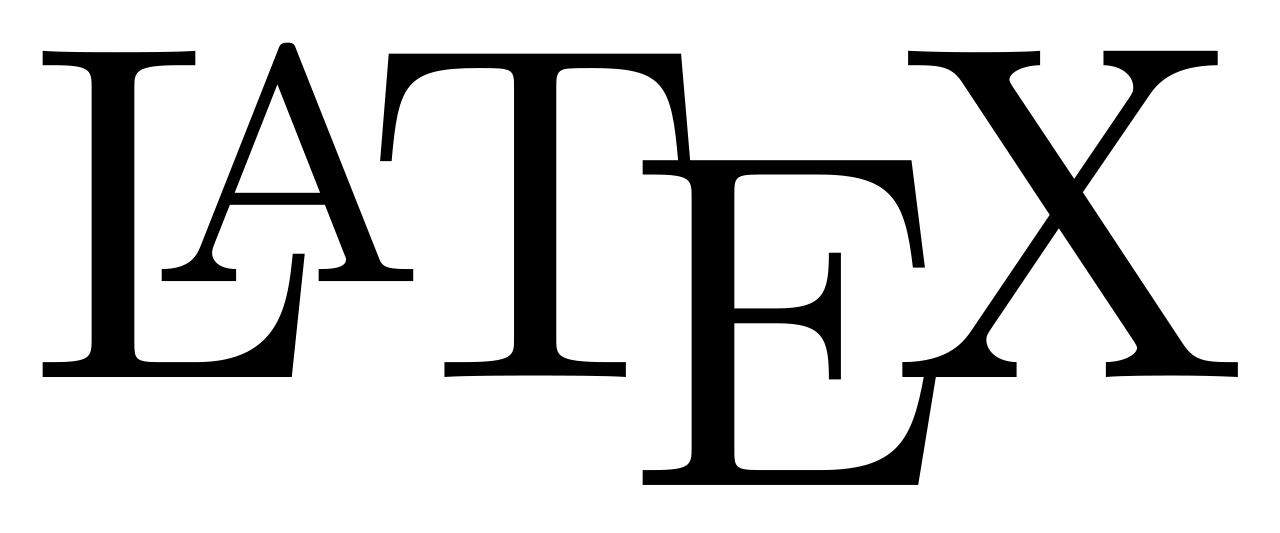
\includegraphics[width=7.5cm]{figs/latex_logo.png}
    \caption{latex logo half}
    \label{fig:latex_logo_half}
  \end{center}
\end{figure}

% This is the figure for twocolumn
\begin{figure*}[t]
\centering
    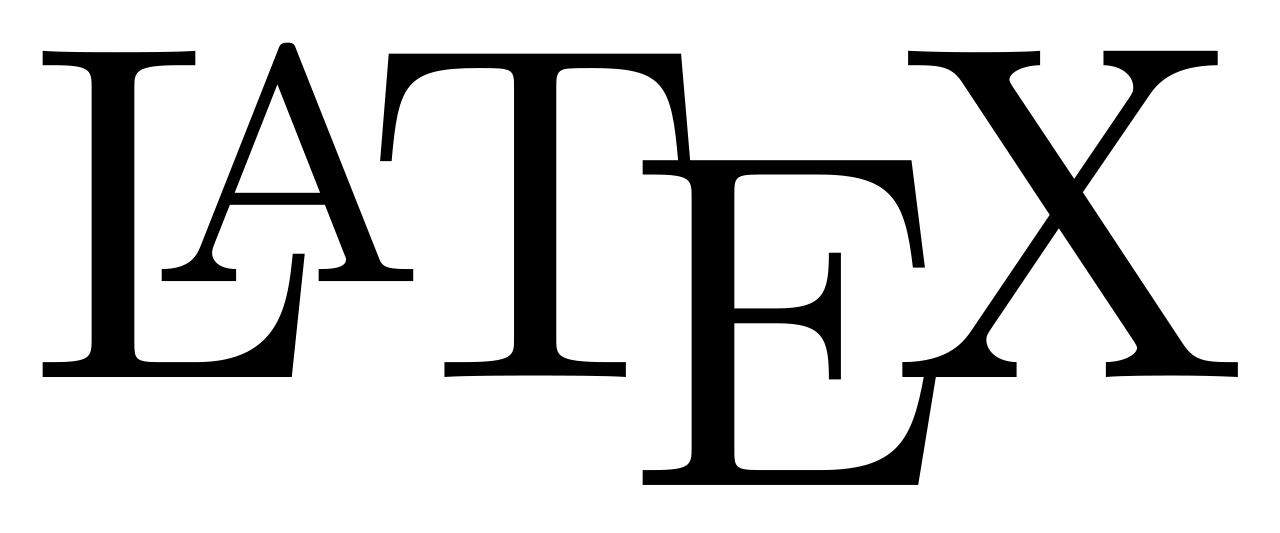
\includegraphics[width=\textwidth]{./figs/latex_logo.png}
    \caption{latex logo}
    \label{fig:latex_logo}
\end{figure*}

% Table
\begin{table}[t]
    \centering
\caption{Quantitative Comparison}
\label{tab:quantitative_eval}
\begin{tabular}{ccccc}
    \toprule
& MethodA & MethodB & Ours \\
    \midrule
MetricsA & 123.5 & 126.9 & {\bf 142.1} \\
MetricsB & 0.887 & 0.910 & {\bf 0.956} \\
\bottomrule
\end{tabular}
\end{table}

\section{Figure, Table, and Equation}
\figref{fig:latex_logo} is the wide figure.
\figref{fig:latex_logo_half} is the small figure.
Table is \tabref{tab:quantitative_eval}.
You can insert the equations like the following.
%
% Equation
\begin{equation}
\label{eq:gauss}
f(x | \mu, \sigma^2) = \frac{1}{\sqrt{2 \pi \sigma^2}} e^{-\frac{(x - u)^2}{2 \sigma^2}}
\end{equation}
You can refer the the above equation \equref{eq:gauss}.
%
You can also refer the other paper which is defined in ref.bib file \cite{goodfellow2014generative}.